\chapter{Applications} \label{chap:App}

\section{Risks measures}

In this section we discuss different ways of measuring the risk of a portfolio.
\begin{definition}
	A portfolio with $n$ assets, $A_1, A_2, \dots, A_n$, is a vector $x^\top = (x_1, x_2, \dots, x_n)\in \R^n$ where each coordinate $x_i$ is the weight of capital invested in asset $A_i$.
\end{definition}
In finance Risk is the probability of losing capital. Considering the loss as a random variable we can calculate the standard deviation of its distribution. This standard deviation (or \textit{volatility}) was considered a measure of risk by Nobel laureate in economics, Harry Markowitz in 1952 (see \cite{Markowitz1952}) under the hypothesis of loss has a normal distribution.

Others risk measures are done in terms of loss distribution percentiles. An upper percentile of the loss distribution is called \textit{Value-at-Risk} ($\mbox{VaR}_\beta$)\footnote{$\mbox{VaR}_\beta$ is the percentile of the loss distribution, i.e., with a specified confidence level $\beta$,  $\mbox{VaR}_\beta$ is the lowest amount $\zeta$ such that, with probability $\beta$, the loss is less or equal to $\zeta$.}. For instance, $\mbox{VaR}_{0.95}$ is an upper estimate of losses which is exceeded with 5\% probability. The popularity of $\mbox{VaR}_\beta$ is mostly related to a simple and easy to understand representation of high losses. $\mbox{VaR}_\beta$ can be quite efficiently estimated and managed when underlying risk factors are normally (log-normally) distributed.

An alternative measure of losses is another percentile risk measure which is called \textit{Conditional Value-at-Risk} ($\mbox{CVaR}_\beta$)\footnote{$\mbox{CVaR}_\beta$ is the average loss in the $100(1-\beta)$\% worst case scenarios.}. The $\mbox{CVaR}_\beta$ risk measure is closely related to $\mbox{VaR}_\beta$. For continuous distributions, $\mbox{CVaR}_\beta$ is defined as the conditional expected loss under the condition that it exceeds $\mbox{VaR}_\beta$, see Rockafellar and Uryasev (see \cite{RockafellarUryasev2001}). For continuous distributions, this risk measure also is known as \emph{Expected Shortfall}, \textit{Mean Excess Loss}, \textit{Mean Shortfall}, or \textit{Tail Value-at-Risk}.


\begin{figure}[!h]
	\centering
	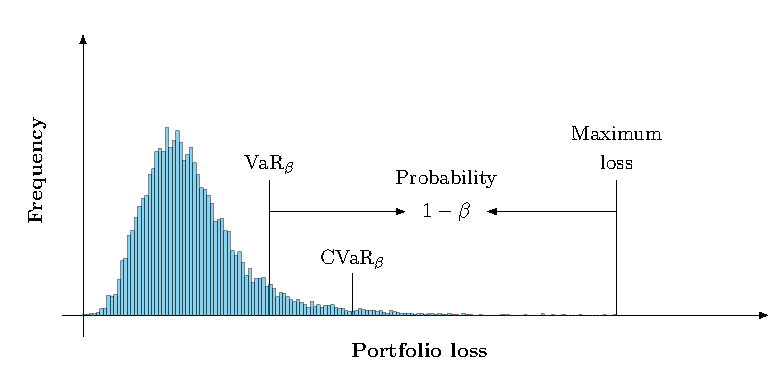
\includegraphics{figures/VarCvar.pdf}
	\caption{Portfolio Loss Distribution, VaR and CVaR.}
	\label{fig:VarCvar}
\end{figure}

\begin{remark}\normalfont\label{re:Normal}
If the loss distribution of a portfolio $x$ is normal, it follows that both $\mbox{VaR}_\beta$ and $\mbox{CVaR}_\beta$ can be rewritten by
\[
	\mu(x)+c\sigma(x)
\]
where $\mu(x)$ and $\sigma(x)$ denote the mean and volatility of the loss associated with portfolio $x$, and $c$ is a constant (see \cite[Chapter 2]{Roncalli2014}). If the portfolio manager has very optimistic forecasts, component $\mu(x)$ may substantially reduce the risk measure. This explains why omitting the mean component is standard practice in the asset management industry.
\end{remark}
% \begin{example}\normalfont
% 	We consider three stocks $A$, $B$ and $C$ whose current prices are respectively $\$ 15.00$, $\$ 25.00$ and $\$ 30.00$. We assume that their expected returns are equal to $30$ bps\footnote{1 bps or one basis point is equivalent to
% 		0.01\% (the hundredth part of 1\%) or 0.0001 in decimal form.}, $50$ bps and $20$ bps on a daily basis and their daily volatilities are $3\%$, $2\%$, and $1\%$ respectively. The asset correlation matrix is given by
% 	\[
% 		\rho = \left(
% 		\begin{array}{rrr}
% 				1.00 & 0.40 & 0.15 \\
% 				0.40 & 1.00 & 0.60 \\
% 				0.15 & 0.60 & 1.00
% 			\end{array}
% 		\right)
% 	\]

% 	We consider a portfolio composed by $100$ stocks $A$, $200$ stocks $B$ and $100$ stocks $C$. The value of this portfolio is $\$ 9,500.00$, being $\$ 1,500.00$ invested in stock $A$, $\$ 5,000.00$ in stock $B$ and $\$ 3,000.00$ in stock $C$, therefore the weights of the stocks in this portfolio are $15.79\%$, $52.63\%$, and $31.58\%$ respectively, so $x=(0.1579;\;0.5263;\; 0.3158)$. The expected loss of the portfolio is $\mu(x) = -30\times0.1579+50\times0.5263+20\times0.3158$, that is, $\mu(x) = -37$ bps. Using the relationship $\Sigma_{i,j}=\rho_{i,j}\sigma_1\sigma_j$ we find the covariance matrix
% 	\[
% 		\Sigma = \left(
% 		\begin{array}{llr}
% 				9.0 & 2.4 & 4.5 \\
% 				2.4 & 4.0 & 1.2 \\
% 				4.5 & 1.2 & 1.0
% 			\end{array}
% 		\right)\times10^{-4},
% 	\] since the volatility of portfolio is given by $\sigma^2(x) = x^\top \Sigma x$, we have that $\sigma(x) = 1.51\%$.

% 	Considering $\alpha = 0.99$, we have $\Phi^{-1}(0.99) = 2.325$ and
% 	$\phi(\Phi^{-1}(0.99))=\phi(2.325)=2.68\%$. Using the equations
% 	$(\ref{eq:var2})$ and $(\ref{eq:cvar2})$ we have

% 	\[
% 		\begin{aligned}
% 			\mathrm{VaR}_{99\%}(x) & = -0.37\% + 2.325 \times 1.51\% = 3.14\%              \\
% 			\mathrm{ES}_{99\%}(x)  & = -0.37\% + \frac{2.68}{0.01} \times 1.51\% = 3.68\%.
% 		\end{aligned}
% 	\]

% 	Risk can also be expressed in monetary terms, in this case,

% 	\[
% 		\begin{aligned}
% 			\mathrm{VaR}_{99\%}(x) & = 3.14\% \times \$ 9,500.00 = \$ 298.30  \\
% 			\mathrm{ES}_{99\%}(x)  & = 3.68\% \times \$ 9,500.00 = \$ 349.60.
% 		\end{aligned}
% 	\]
% 	According to the result of {\rm VaR}, in $99\%$ of the days, the loss will be less than $\$ 298.30$, however in the $1\%$ of the remaining days the {\rm VaR} does not measure how much great can be the loss, this is the role of {\rm CVaR} which indicates that the average loss will be $\$ 349.60$ on the worst $1\%$ days.
% \end{example}


\section{Portfolio optimization}

In this section we present some ways to build a portfolio. In a universe of $n$ assets let $x^\top = (x_1, x_2, \dots, x_n)$ be a portfolio and denoting by $R_i$ the return of asset $i$. If $R^\top=(R_1, R_2, \dots, R_n)$  is the random vector of asset returns then the return of portfolio $x$ is given by:
\[
	R(x) = x_1R_1+x_2R_2+\cdots x_nR_n = x^\top R.
\]
If we denote by $\mu$ and $\Sigma$ the vector of expected returns and the covariance matrix of asset returns respectively, we deduce that the expected return of portfolio $x$ is equal to:
\[
	\mu(x) = x^\top \mu
\]
whereas its variance is given by:
\[
	\sigma^2(x) = x^\top \Sigma x.
\]
The mean-variance portfolio (MVP) of Markowitz (see \cite{Markowitz1952}) consists in maximizing the expected return $\mu(x)$ for a fixed value $\nu$ of the volatility $\sigma(x)$. This can be achieved by solving the problem:
\begin{eqnarray}\label{prob:MVP}
	\min_{x} \, \{- \mu(x)\}, \\
	\mbox{s.t. }\left\{
	\begin{aligned}\nonumber
		\sigma^2(x) = \nu, & \\
		\mathbf{1}^\top x=1       &
	\end{aligned}
	\right.
\end{eqnarray}
where $\textbf{1}^\top =(1,1,\dots,1)$, and the condition $\mathbf{1}^\top x=1$ means that the capital is fully invested.

A portfolio optimization  problem is defined when we want to minimize (or maximize) a performance measure subject to a set of constraints. Here are some examples of performance measures and constraints:

\begin{itemize}
	\item \textbf{Performance Measures}
	      \begin{itemize}
		      \item Expected return: $\mu(x)$;
		      \item Volatility: $\sigma(x)$;
		      \item Sharpe Ratio (SR): expected return per unit of risk
		            \[
			            \mbox{SR}(x) = \frac{x^\top \mu - r_f}{\sigma(x)}
		            \]
		            where $r_f$ is the risk-free rate (e.g. interest rate on a Treasury bill);
		      \item Information Ratio (IR): Sharpe Ratio with $r_f=0$;
		      \item $\mbox{VaR}_\beta$ (Value at Risk): quantile of the loss;
		      \item $\mbox{CVaR}_\beta$ (Conditional Value at Risk): expected value of the loss above some quantile.
	      \end{itemize}
\end{itemize}

\begin{itemize}
	\item \textbf{Constraints}
	      \begin{itemize}
		      \item Capital constraint: $\textbf{1}^\top x=1$;
		      \item Long-only constraint: $x\geq0$;
		      \item Self-financial constraint: $\textbf{1}^\top x=0$;
		      \item Holding constraint: $\mathbf{I}\leq x\leq \mathbf{J}$ where $\mathbf{I},\mathbf{J}\in\R^n$ are lower and upper bounds of the asset positions, respectively.
		      \item Leverage constraint: $\|x\|_1\leq K$.
	      \end{itemize}
\end{itemize}

Some known portfolio optimization problems are:

\noindent\textbf{Minimum Variance Portfolio (MVP)}

Minimize variance with fully capital invested
\begin{eqnarray}\label{eq:MVP}
	\min_{x} \,\big\{x^\top \Sigma x\big\}, \\
	\mbox{s.t. }\left\{
	\begin{aligned}\nonumber
		\mathbf{1}^\top x=1 \\
	\end{aligned}
	\right\}.
\end{eqnarray}

\noindent\textbf{Maximum Sharpe Ratio Portfolio (MSRP)}

Maximize Sharpe ratio with self-financial constraint and leverage restriction.
\begin{eqnarray}\label{prob:MSRP}
	\max_{x} \,\big\{\mbox{SR}(x)\big\}, \\
	\mbox{s.t. }\left\{
	\begin{aligned}\nonumber
		\mathbf{1}^\top x=0, & \\
		\|x\|_1\leq K.
	\end{aligned}
	\right.
\end{eqnarray}

We can also combine performances and constraints like this example:
\begin{eqnarray}\label{prob:General}
	\min_{x} \,\big\{\lambda \mbox{CVaR}_\beta(x) - \mu(x)\big\}, \\
	\mbox{s.t. }\left\{
	\begin{aligned}\nonumber
		\mathbf{1}^\top x=1, & \\
		\|x\|_1\leq K.
	\end{aligned}
	\right.
\end{eqnarray}
where $\lambda$ is a parameter that controls how risk-averse the investor is. 

Furthermore, we can look at portfolio optimization problems as a multi-objective problem: Let $f:\R^n\to\R^2$ be the function $f(x)= \big(\mathcal{P}(x), \mathcal{R}(x)\big)$, where $\mathcal{P}(x)$ is a performance measure (that we want to minimize) of portfolio $x$ and $\mathcal{R}(x)$ is a risk measure of $x$. We want to find a solution to problem
\begin{eqnarray}\label{prob:Vector}
	\min_{x} \,\Big\{f(x)= \big(\mathcal{P}(x), \mathcal{R}(x)\big)\Big\}, \\
	\mbox{s.t. }\left\{
	\begin{aligned}\nonumber
		\mathbf{1}^\top x=1.
	\end{aligned}
	\right.
\end{eqnarray}

In all these problems we want to optimize a performance measure, we will present a new approach where the objective will be the risk allocation.

\section{Risk Parity}

Markowitz’s portfolio has never been fully embraced by practitioners, among other reasons because it only considers the risk of the portfolio as a whole and ignores the diversification risk (i.e., concentrates too much risk in few assets, this was observed in the 2008 financial crisis): one solution to avoid this problem is the risk parity portfolio.

Risk parity is an approach to portfolio management that focuses on allocation of risk rather than allocation of capital. The risk parity approach asserts that when asset allocations are adjusted to the same risk level, the portfolio can achieve a higher Sharpe ratio and can be more resistant to market downturns.

While the minimum variance portfolio tries to minimize the variance (with the disadvantage that a few assets may be the ones contributing most to the risk), the risk parity portfolio distributes the weights so that the risk contribution of each asset (or asset class, such as bonds, stocks, real estate, etc.) is the same.

To define a risk-based allocation strategies it is necessary define how the risk of an asset affects the risk of the portfolio. 
Let $x^\top=(x_1,x_2,\dots,x_n)$ be a portfolio with $n$ assets and $\mathcal{R}(x)$ be a differentiable, homogeneous risk measure of $x$. Since $\mathcal{R}(x)$ is homogeneous, we have
\[
\mathcal{R}(x)=\frac{d}{d\lambda}\mathcal{R}(\lambda x)=\sum_{i=1}^n x_i \frac{\partial \mathcal{R} (x)}{\partial x_i}
\]
we can define the risk contribution of the asset $i$ by
$\mathcal{RC}_i$, where
\[
\mathcal{RC}_i(x)= x_i \frac{\partial \mathcal{R}(x)}{\partial x_i}.
\]
Therefore, the risk can be written as follows
\[
\mathcal{R}(x)=\sum_{i=1}^n \mathcal{RC}_i(x)
\]
which is known as \textbf{Euler's Allocation Principle}.

Volatility and $\mbox{CVaR}_\beta$  satisfy the properties required by the risk measure, $\mathcal{R}$, defined above. However, $\mbox{VaR}_\beta$ satisfies these properties only in the Gaussian case. When asset returns have a Normal Distribution, by simplicity (see Remark \ref{re:Normal}), we have that
$\mathcal{R}(x)=\sigma(x)=\sqrt{x^\top\Sigma x}$, it follows that
\[
\mathcal{RC}_i(x)= x_i \frac{\partial \sigma(x)}{\partial x_i}=\frac{x_i (\Sigma x)_i}{\sqrt{x^\top\Sigma x }}.
\]

It may be interesting for the investor to choose different risks for different assets, in this case the investor choose the percentage of risk that each asset should have in the portfolio, that is,
\begin{equation}\label{eq:RBP}
	\mathcal{RC}_i(x)=b_i\mathcal{R}(x),
\end{equation}
where $b_i$ represents the risk contribution that asset $i$ will have in the portfolio. Certainly $b_i\geq 0$ for all $i$ and
${\bf 1}^\top b =1$, with $b^\top=(b_1, b_2, \dots, b_n)$. A portfolio distribution based in relation \eqref{eq:RBP} is called \textit{risk budgeting portfolio} (RBP), when $b_i=1/n$, for all $i$ the distribution is called \textit{risk parity portfolio} (RPP) or \textit{equal risk portfolio} (ERP).

In general, find the risk budgeting portfolio consists to solve the following non-linear system
\begin{eqnarray}\label{eq:SisNLin}
\mathcal{RC}_i(x)=b_i\mathcal{R}(x), \\
	\mbox{s.t. }\left\{
	\begin{aligned}\nonumber
b_i \geq 0, \\
x_i \geq 0, \\
{\bf 1}^\top b =1, \\
{\bf 1}^\top x =1.
	\end{aligned}
	\right.
\end{eqnarray}

In 2012 Kaya and Lee (see \cite{KayaLee2012}) show that, in Gaussian case, the risk budgeting portfolio can be found by solving the problem
\begin{eqnarray}\label{eq:RPP}
\min_{x\geq \textbf{0}}\, \{-b^\top \ln(x)\}; \\
	\mbox{s.t. }\left\{
	\begin{aligned}\nonumber
\sigma^2(x)\leq \sigma_0,\\
{\bf 1}^\top x =1.
	\end{aligned}
	\right.
\end{eqnarray}
where, $\sigma_0$ is a volatility target.





